\documentclass[journal]{IEEEtran}
% IEEE Transactions on Industrial Informatics -- anonymous regular-paper draft
% Compile: latexmk -pdf main.tex
\usepackage{amsmath,amssymb,amsfonts}
\usepackage{algpseudocode}
% Local XeTeX/Tectonic builds: route IEEEtran's ptm (Times) family requests to
% the legacy Times Type1 faces so metrics match the pdfLaTeX reference build;
% the latexmk -pdf (pdfLaTeX) path is unaffected.
\usepackage{iftex}
\ifxetex
  \DeclareFontFamily{TU}{ptm}{}
  \DeclareFontShape{TU}{ptm}{m}{n}{<->ptmr8t}{}
  \DeclareFontShape{TU}{ptm}{b}{n}{<->ptmb8t}{}
  \DeclareFontShape{TU}{ptm}{m}{it}{<->ptmri8t}{}
  \DeclareFontShape{TU}{ptm}{b}{it}{<->ptmbi8t}{}
  \DeclareFontShape{TU}{ptm}{m}{sl}{<->ptmro8t}{}
  \DeclareFontShape{TU}{ptm}{m}{sc}{<->ptmr8t}{}
\fi
\usepackage{graphicx}
\usepackage{booktabs}
\usepackage{tabularx}
\usepackage{array}
\usepackage[table]{xcolor}
\usepackage{stfloats}
\usepackage{placeins}
\usepackage{url}
% Allow line breaks at any character inside URLs/DOIs so long reference links
% do not leave ragged gaps at column edges (IEEE reference layout).
\usepackage{xurl}
\usepackage{etoolbox}
\urlstyle{same}
% Cross-references and citations. The cite package renders IEEE-style citation
% groups ([14]--[16], [20], [21]) with hyperref support.
\usepackage{cite}
\usepackage[colorlinks=true,linkcolor=black,citecolor=black,urlcolor=black]{hyperref}
\hypersetup{bookmarksnumbered=true,
  pdftitle={A Configuration-Driven Runtime for Integrating Industrial Agents With Online Data Acquisition and Governed Setpoint Operations},
  pdfauthor={},
  pdfsubject={IEEE Transactions on Industrial Informatics},
  pdfkeywords={industrial agents, industrial communication, online data acquisition, setpoint governance}}

% Float placement only; IEEEtran margins and body type remain unchanged.
\setcounter{topnumber}{4}
\setcounter{bottomnumber}{3}
\setcounter{totalnumber}{7}
\setcounter{dbltopnumber}{1}
\renewcommand{\topfraction}{0.95}
\renewcommand{\bottomfraction}{0.80}
\renewcommand{\textfraction}{0.03}
\renewcommand{\floatpagefraction}{0.72}
\renewcommand{\dbltopfraction}{0.95}
\renewcommand{\dblfloatpagefraction}{0.72}

% Tight but conventional float separation; body type and margins are unchanged.
\setlength{\textfloatsep}{8pt plus 2pt minus 3pt}
\setlength{\dbltextfloatsep}{8pt plus 2pt minus 3pt}
\setlength{\intextsep}{7pt plus 2pt minus 3pt}
\setlength{\abovecaptionskip}{3pt plus 1pt minus 1pt}
\setlength{\belowcaptionskip}{2pt plus 1pt minus 1pt}

\newcommand{\system}{the platform}

\begin{document}
\bstctlcite{IEEEbstctl}

\title{A Configuration-Driven Runtime for Integrating Industrial Agents With Online Data Acquisition and Governed Setpoint Operations}

\author{}
\markboth{IEEE Transactions on Industrial Informatics, Submitted Manuscript}{Agent-Mediated Setpoint Control}

\maketitle

\begin{abstract}
An industrial agent needs process measurements to propose a setpoint change and a governed route to execute it. We present a configuration-driven runtime that maps acquisition and control signals separately for each production scene. Task-mediated and direct tool calls share a dispatcher. The operation handler checks authorization and write limits and revalidates approved requests before dispatch. Command outcomes, setpoint readbacks, and subsequent process measurements are recorded separately. At 55 endpoints across four simulated scenes and five protocols, the node-write service accepted all 220 admissible requests and rejected all 219 hard-range probes and 110 recipe-window probes. All 216 follow-up reads matched the requested simulator setpoints. In an injection simulator, a governed write changed holding pressure from 60 to 63.7 bar with matching readback. In a separate exploratory comparison across injection molding, wastewater treatment, and annealing, a scripted policy yielded lower integrated absolute error than no-write in all nine valid pairs in the reported batch. Three language-model-driven injection runs issued two-parameter trials and ended below target. The experiments demonstrate governed writes in simulation and identify the remaining gap in autonomous execution.
\end{abstract}

\begin{IEEEkeywords}
Industrial agents, industrial communication, online data acquisition, setpoint governance.
\end{IEEEkeywords}

\IEEEpeerreviewmaketitle

\section{Introduction}
\IEEEPARstart{A}{n} industrial agent that proposes a setpoint change must know which signal to read, which node to write, and which limits govern the write. On a cast-film line, for example, the agent can compare measured thickness with a production target and propose a speed adjustment. The thickness and speed signals use separate mappings even when both travel over Message Queuing Telemetry Transport (MQTT). The runtime must resolve the control node, check the caller's authority, and record what happened after the command. Fig.~\ref{fig:control-path} illustrates this sequence.

Industrial-agent research addresses service supervision, skill-based manufacturing, and fault recovery \cite{biskupovic2025supervision,koehle2026llmdriven,vyas2026detection}. Studies of programmable logic controller (PLC) integration also examine semantic grounding, approval, and proposal verification \cite{graul2026aas,schall2026safe}. We ask how one runtime can carry production context from acquisition to a governed setpoint operation when a task agent or a direct tool caller initiates the request.

We use the term \emph{production scene} for the configuration that links the line, product, recipe, and run to node mappings, drivers, objectives, and limits. The agent uses this context to select observations and propose a typed adjustment. The runtime checks the operation against live authority and limits, revalidates approved requests, and retains the command result separately from the setpoint readback and later process measurements.

The contributions are:
\begin{enumerate}
  \item A scene configuration that maps acquisition and control signals to registered drivers and supplies operating context to the runtime (Section~\ref{sec:design}).
  \item A shared dispatcher and governed operation handlers that connect agent tool calls to conditional approval, setpoint dispatch, and verification records (Sections~\ref{sec:design}--\ref{sec:modules}).
  \item An evaluation of setpoint writes and readbacks across four simulated scenes, with targeted checks of approval and guard behavior and an exploratory comparison of process trajectories under scripted writes and no-write (Section~\ref{sec:eval}).
\end{enumerate}

\begin{figure}[!b]
\centering
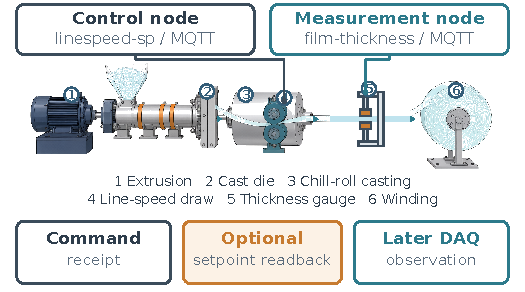
\includegraphics[width=0.98\columnwidth]{resources/fig1-vectorized-20261109.pdf}
\caption{Cast-film example. The agent reads film thickness and can propose a line-speed adjustment. The acquisition and control nodes have separate MQTT mappings. Command acceptance, setpoint readback, and later thickness measurements describe different stages of the operation.}
\label{fig:control-path}
\end{figure}



\section{Related Work}
\label{sec:related}
Table~\ref{tab:related-comparison} summarizes representative systems and their evaluation settings.

\begin{table*}[!t]
\centering
\caption{Representative industrial-agent systems and the scope of their evaluations. OPC UA denotes Open Platform Communications Unified Architecture.}
\label{tab:related-comparison}
\footnotesize
\setlength{\tabcolsep}{5pt}
\begin{tabularx}{\textwidth}{@{}>{\raggedright\arraybackslash}p{0.16\textwidth}>{\raggedright\arraybackslash}p{0.40\textwidth}X@{}}
\toprule
Study & Main focus & Reported setting \\
\midrule
Biskupovic et al.~\cite{biskupovic2025supervision} & Agent-based industrial service selection and reselection & Service adaptability and performance in an industrial cyber--physical system \\
K\"{o}hle et al.~\cite{koehle2026llmdriven} & Module-specific agents and skill-based manufacturing & Nine simulated production challenges \\
Graul et al.~\cite{graul2026aas} & Grounded proposals, documented authorization, and proposed PLC-side checks & Two proof-of-concept scenarios using a simulated OPC UA server \\
Schall~\cite{schall2026safe} & Process-diagram, supervisory control and data acquisition (SCADA), and procedure-grounded verification & Five simulated scenarios and proposal evaluation \\
Vyas et al.~\cite{vyas2026detection} & Multi-agent fault-recovery planning with a process-plant twin & Simulated mixing and stirred-tank reactor studies \\
This work & Scene-bound signal mappings, shared dispatch, and route-specific governance & Simulator and mock-driver probes, scripted trials, and exploratory language-model runs \\
\bottomrule
\end{tabularx}
\end{table*}

\subsection{Industrial Agents and Plant Integration}
Biskupovic et al. study online service selection and reselection in industrial cyber--physical systems \cite{biskupovic2025supervision}. Xia et al. present a digital-twin-connected automation architecture and control generation \cite{xia2025architecture,xia2025control}; other work generates PLC programs \cite{liu2026agents4plc}. In related control research, human instructions have also been incorporated into model-predictive control \cite{wu2025instructmpc}.

Li et al. use structured instructions, retrieval, and iterative verification to generate and check finite-element scripts for Abaqus; that study evaluates engineering-artifact generation rather than runtime authority over process writes \cite{li2026modsolagent}. Other studies examine large language model (LLM) agents, manufacturing skills, and natural-language machine interaction \cite{koehle2026llmdriven,lim2025llmenabled,zhao2026shopfloor,hofmann2025nlc}. Vyas et al. combine multi-agent fault-recovery planning and plant-knowledge retrieval with Digital Process Plant Twin studies of mixing and continuous stirred-tank reactors (CSTRs) \cite{vyas2026detection}.

These studies address how agents select services, compose actions, or generate control logic. Our implementation addresses how the resulting operation resolves a scene-specific signal and its write constraints at dispatch time.

\subsection{Industrial Interfaces and Semantic Commissioning}
Agent-facing interfaces use the Model Context Protocol (MCP) to expose manufacturing resources \cite{silva2025mcpmanufacturing}, Open Platform Communications Unified Architecture (OPC UA) skills to compose semantic recipes \cite{koehle2025semanticrecipes}, and protocol adapters to access equipment \cite{xavier2026industriConnect}. Semantic commissioning also connects manufacturing data to cognitive digital twins \cite{liu2026semanticcommissioning}. Our runtime uses configured bindings to resolve read and write nodes, then enforces authorization and value limits in the operation service.

\subsection{Governed Operations and Verification}
Graul et al. ground plans in the Asset Administration Shell and propose documented human authorization and PLC-side validation of OPC UA Methods \cite{graul2026aas}. Schall verifies proposals against piping and instrumentation diagrams, supervisory control and data acquisition (SCADA) data, and operating procedures \cite{schall2026safe}. Lin and Chen describe a policy-governed digital thread spanning sensors, manufacturing execution systems (MES), and enterprise resource planning \cite{lin2026agentic}. PLCBench evaluates autonomous agents against commercial PLCs coupled to a process simulator \cite{zhou2026plcbench}. The focus here is application-level execution across registered industrial protocols, including what the runtime records at approval, dispatch, and verification.

\subsection{Production Context and Outcome Evidence}
MCP standardizes tool discovery and invocation \cite{mcp2026}, while ISA-88 and ISA-95 define recipe and production-operation concepts \cite{isa88_2010,isa95_2025}. Run-to-run control connects observations to subsequent decisions, and human--automation research examines how to allocate responsibilities between people and automated systems \cite{moyne2001r2r,parasuraman2000model}. The operation contract described next connects these concerns at the write boundary by resolving scene context, checking the caller's authority, and returning a record the caller can use before deciding on another operation.

\section{System Design}
\label{sec:design}
The runtime exposes named operations through two entry paths. In a task, a registered harness gives the agent scoped tools to read process data and submit a proposed change. External callers can invoke the same tools through the Representational State Transfer (REST) interface or the standard-I/O MCP bridge. Both paths enter the shared dispatcher. Scene configuration supplies the production context and the mappings and limits the handlers use.

\begin{figure*}[!t]
\centering
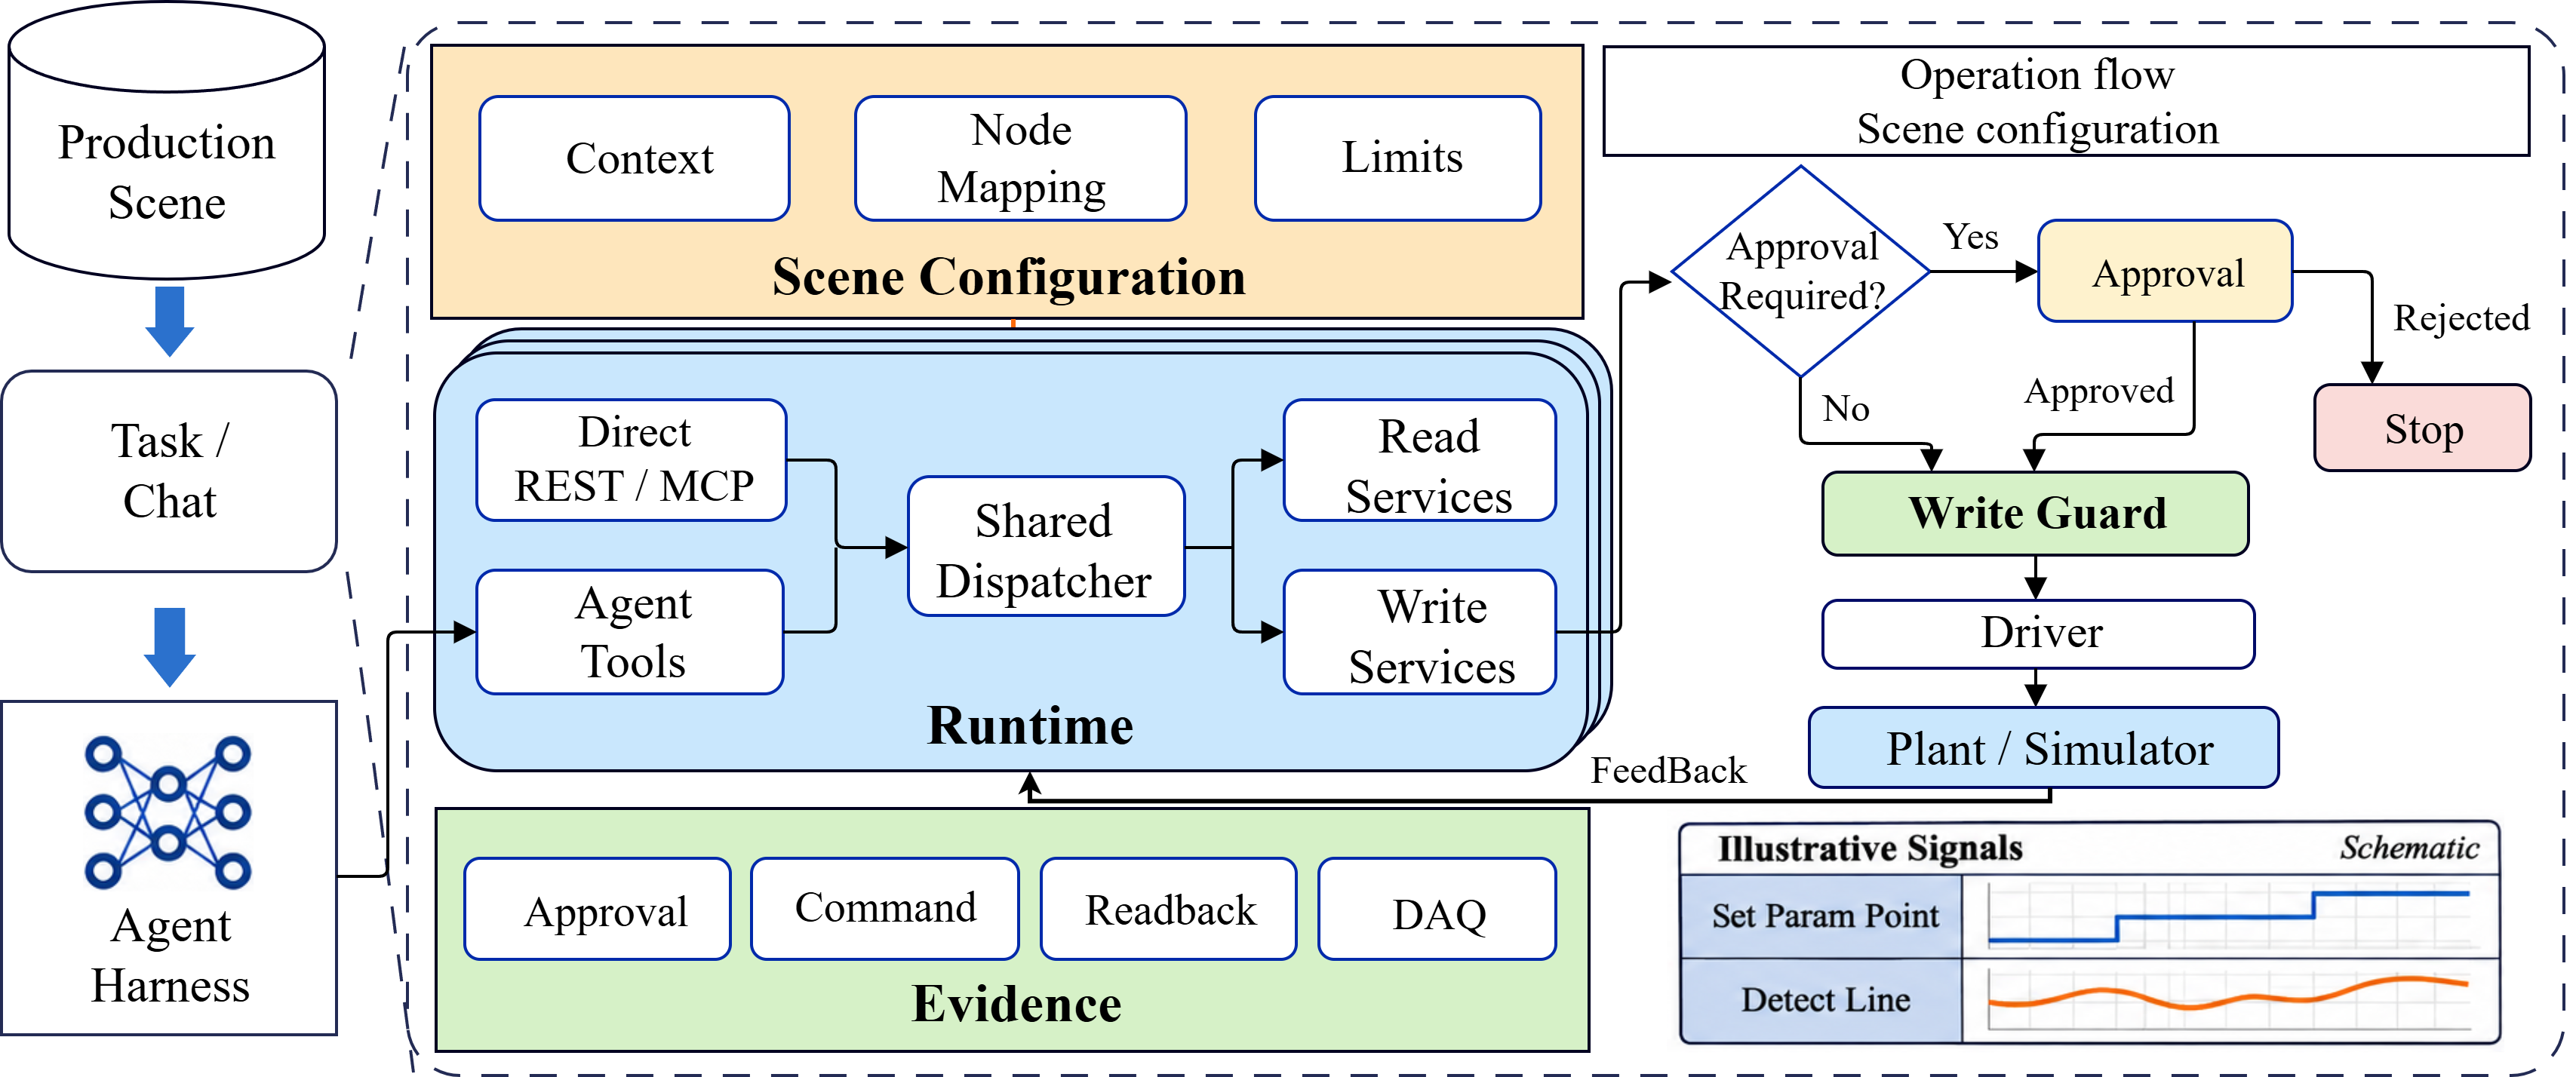
\includegraphics[width=\textwidth]{resources/fig2.png}
\caption{Scene configuration, shared dispatch, and governed write execution. Task-mediated and direct tool calls reach the same dispatcher. Every write follows the applicable authorization and guard checks. A required approval triggers route-specific revalidation (Fig.~\ref{fig:hitl}). Only an admitted command reaches the driver. Approval, command outcome, optional readback, and subsequent data acquisition (DAQ) produce separate records. The inset illustrates setpoint and process signals schematically.}
\label{fig:arch}
\end{figure*}

\subsection{Design Rationale and Requirements}
\label{sec:principles}
The agent uses production context and available observations to decide what to propose. The operation handler determines whether it can execute that proposal against the current state. Keeping those decisions separate lets the harness present the same tools across scenes while the runtime checks the applicable node bindings, authority, and limits for each write.

\subsection{Layered Architecture}
\label{sec:layers}
Fig.~\ref{fig:arch} shows how task and chat calls enter the runtime through a harness, while direct tool calls reach the dispatcher without a task. The dispatcher routes reads to DAQ, MES access, retrieval, or other analysis services and writes to node or recipe services. The services use configured input and output mappings to reach built-in or plugin drivers. The administrative node-write interface used in Section~\ref{sec:eval-mapping} exercises the downstream write controller independently of task and agent-tool dispatch.

\subsection{Scene Configuration as the Integration Boundary}
\label{sec:scene-config}
The active line identifies the production context. Product and recipe records supply targets and limits, and the run record supplies the operating state. Each semantic node names a process variable and specifies its direction, unit, and mapping. The registry resolves that mapping to a registered driver. The harness calls a named, typed operation without constructing a protocol message. A new scene can bind existing drivers through configuration. Adding support for another protocol requires a driver adapter.

In the cast-film simulator preset, for example, the MQTT command mapping
\texttt{linespeed-sp} controls line speed in m/min, while the distinct
\texttt{film-thickness} mapping supplies thickness in $\mu$m. An agent can
acquire the thickness observation, compare it with its objective, and propose a
line-speed adjustment. The runtime checks the proposal against the speed node's
limits and sends an admitted command to its MQTT mapping.

Table~\ref{tab:scene-config} shows where the runtime uses each configuration element. Before dispatch, the handler resolves the live state required by its route. Recipe operations bind approval to both the proposal and the active production context.

\begin{table*}[!t]
\centering
\caption{Scene configuration elements and their roles in the runtime path.}
\label{tab:scene-config}
\footnotesize
\setlength{\tabcolsep}{5pt}
\begin{tabularx}{\textwidth}{@{}>{\raggedright\arraybackslash}p{0.19\textwidth}>{\raggedright\arraybackslash}p{0.34\textwidth}X@{}}
\toprule
Element & Configured information & Runtime use\\
\midrule
Production context & Line, product, recipe, and run associations & Context construction for a task turn; route-dependent live-state checks before a write\\
Semantic I/O & Process variable, direction, unit, and node mapping & Acquisition uses the read mapping; accepted operations resolve the configured control mapping\\
Driver binding & Supported protocol driver and endpoint configuration & Driver registry selects the protocol implementation after operation checks\\
Operation admission & Engineering, baseline, product, and recipe limits; step and timing rules where configured & Route handler checks the candidate against current bounds and rejects inadmissible requests\\
Approval policy & Whether approval is required and the decision validity window & Pending request binds the proposed action; route-specific checks run after approval\\
Evidence ownership & Command receipt, verification grade, and later DAQ observations & Owning services retain command outcomes separately from process measurements\\
\bottomrule
\end{tabularx}
\end{table*}

\subsection{Cross-Module Execution Flow}
\label{sec:executionflow}
For a task-mediated call, the registered adapter presents a scoped tool
catalog containing acquisition, context, and control operations to the agent.
The agent reads available observations, relates them to the task objective, and
submits a typed intent rather than a protocol-specific message. At the
operation boundary, the shared dispatcher checks the predicates declared for
the named operation before selecting its handler. The handler resolves live
production state, applies route-specific guards and limits, and requests any
required approval before device I/O.

For an industrial operation $u$ by agent $a$ in channel $c$, define the
shared dispatch condition as
\begin{equation}
\mathcal{A}(a,c,u)=\bigwedge_{X\in\mathcal{C}(u)}X(a,c,u).
\label{eq:dispatch-contract}
\end{equation}
In Eq.~(\ref{eq:dispatch-contract}), $S$, $P$, $G$, and $B$ denote invocation scope, current channel policy,
applicable industrial grant, and the agent's binding to referenced resources,
respectively. $\mathcal{C}(u)\subseteq\{S,P,G,B\}$ is the set of predicates
declared for operation $u$; it always contains $S$ and $P$. The grant predicate
$G$ is included when the resolved channel, target line, and owner/grant policy
require it; explicit exemptions omit it. The binding predicate $B$ is included
when the operation declares resource references. An operation that declares
no references omits $B$. Each included check must pass before handler
selection. The policy predicate includes channel tool selection, profile, and duty-separation checks where
configured.

Once these predicates pass, the selected route applies its operational
guards and requests any required approval. For example, an exploration request checks
the control binding and DAQ visibility before entering the governed write
path; an invisible target returns an error before a write. The checks performed
after approval depend on the route; Section~\ref{sec:modules} specifies the
single-node and recipe-operation paths.

For a direct REST agent-tool call, the service establishes $a$ and $c$ before applying
these checks. An agent token must match the requested agent identifier; an
authenticated user must be the channel owner or an administrator. The manager
loads the channel-agent record and rechecks scope and policy, followed by any
applicable grant and binding checks. Handlers resolve live production state
using request identifiers and the owning services.



\section{Agent-Coordinated Task-Level Operation}
\label{sec:closed-loop-operation}

\begin{figure*}[!t]
\centering
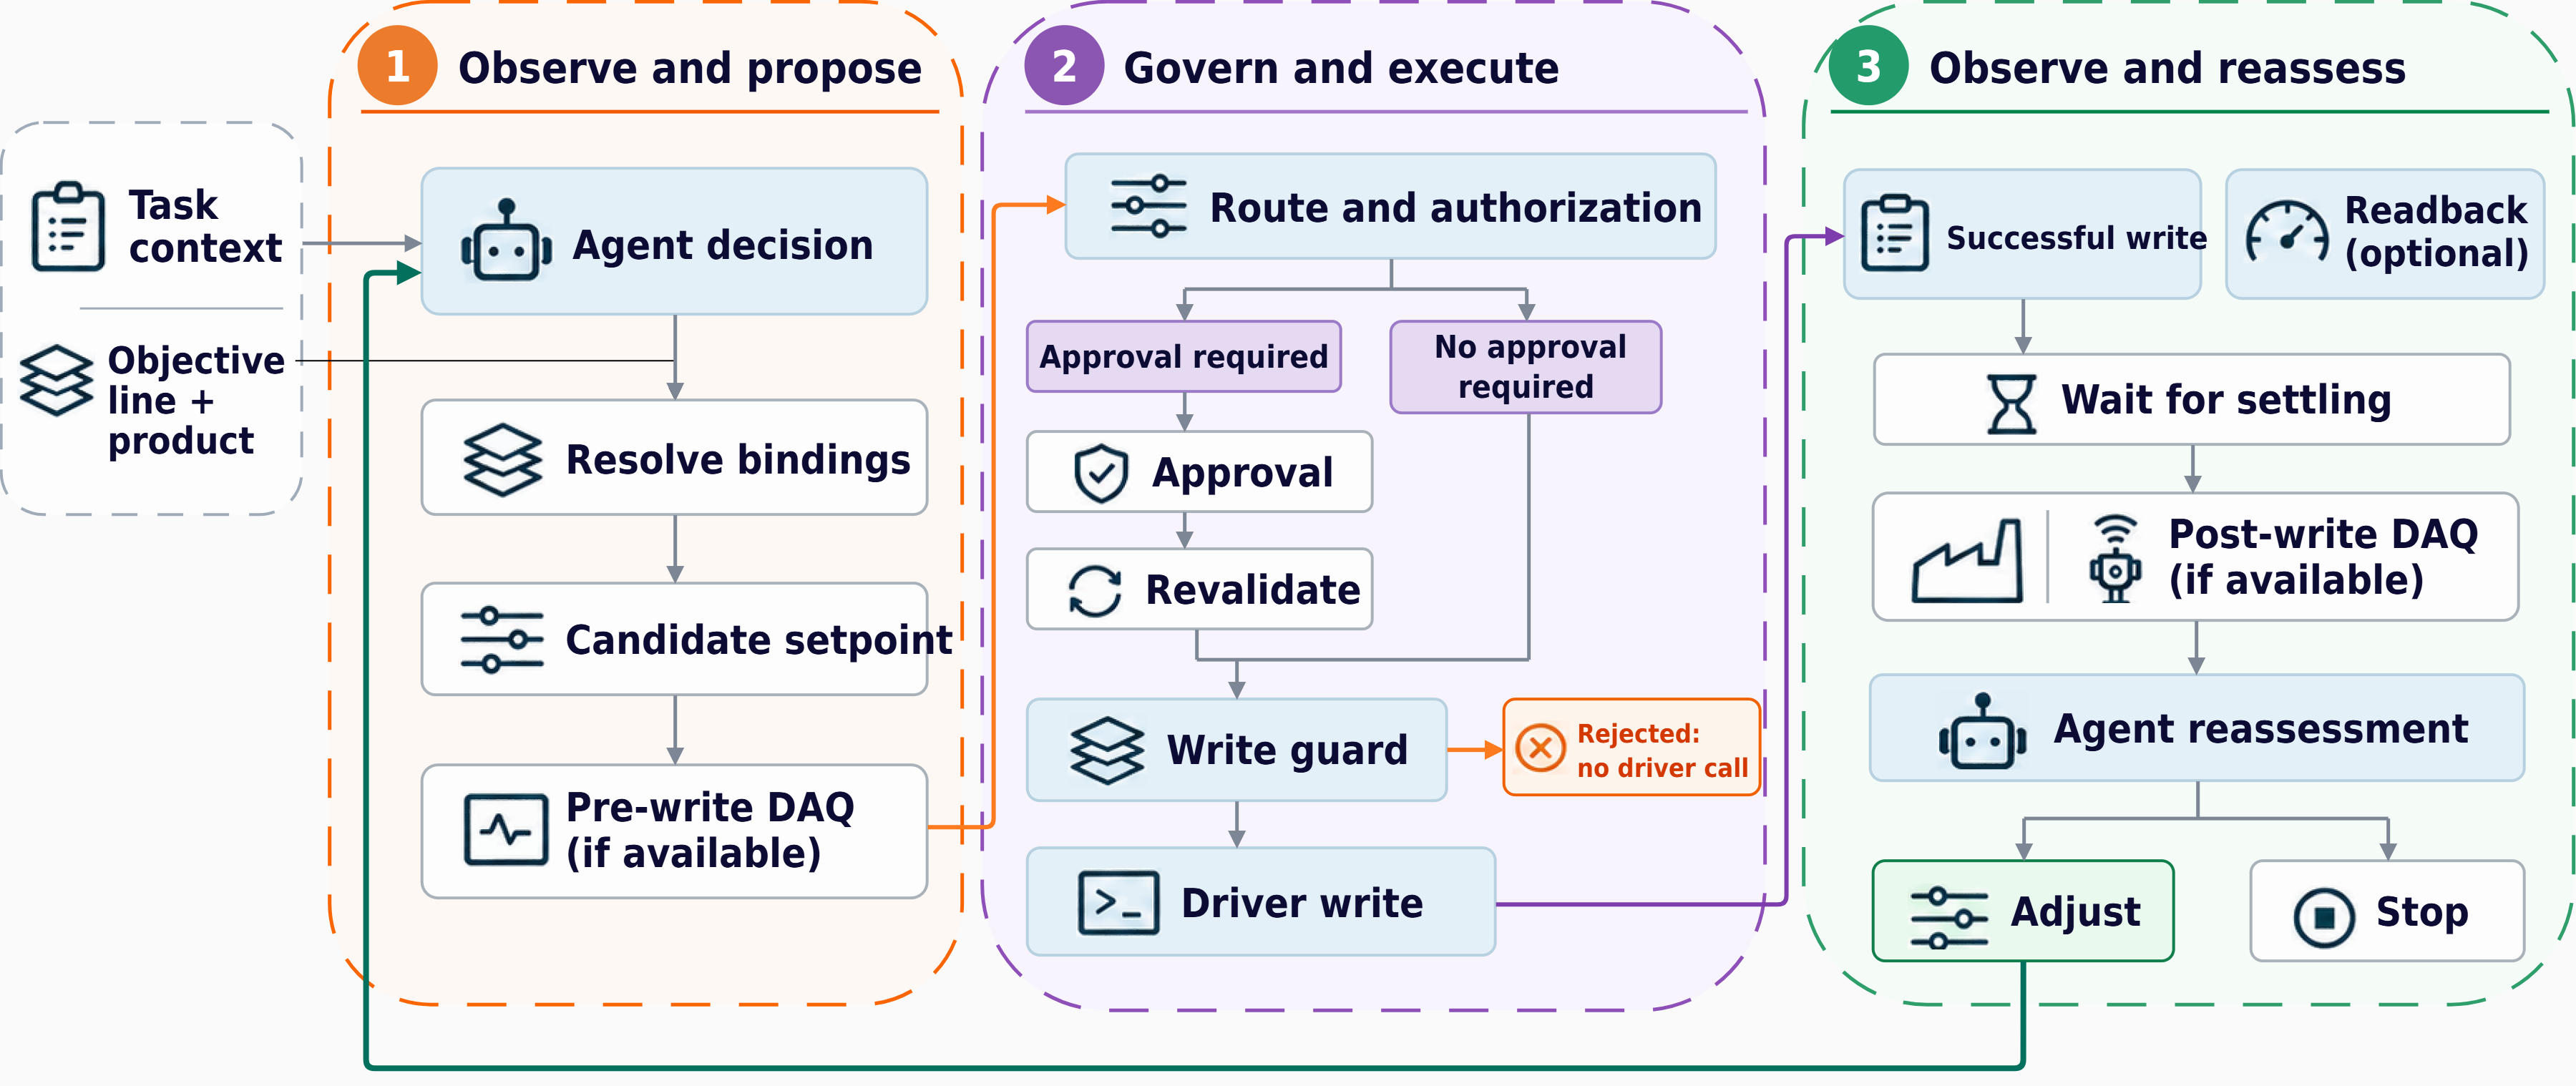
\includegraphics[width=\textwidth]{resources/fig3.png}
\caption{Agent-coordinated task workflow. The agent uses available observations to propose a setpoint. The runtime checks admission before driver dispatch and returns the command outcome, optional readback, and later DAQ observations for reassessment. The diagram shows the workflow design. Fig.~\ref{fig:hitl} details the conditional approval path.}
\label{fig:agent-loop}
\end{figure*}

A task supplies an objective and production context. The agent can acquire configured observations, compare them with the objective, and submit a typed adjustment. The workflow in Fig.~\ref{fig:agent-loop} returns operation results to the agent for the next decision. The caller can identify the control node and DAQ target explicitly. The operation uses their respective bindings when the caller omits them.

In goal mode, a lead agent can decompose the objective and assign worker subtasks. A worker can call \texttt{optimization\_explore} to request a single-node adjustment and collect process measurements around it.

In the evaluated version, the operation resolves the profile and control binding and uses the stored setpoint as $u_0$. Given a direction $s\in\{-1,+1\}$ and step $\Delta u$, it forms
\begin{equation}
 u^{*}=\operatorname{clip}\!\left(u_0+s\Delta u,\,u_{\min},\,u_{\max}\right).
 \label{eq:optimization-candidate}
\end{equation}
The operation defaults to increasing the value when no direction is supplied. In Eq.~(\ref{eq:optimization-candidate}), it clips the candidate to the configured tuning bounds or, if absent, the node bounds. It selects the step from the first available source among the explicit argument, binding, and scene limit. The default is one twentieth of the node range.

Before submitting the candidate, the operation checks that the DAQ target is visible to the caller and attempts a pre-write read. Identifiability and model--ontology checks were added after the experiments.

A valid candidate enters the governed write path in Algorithm~1. A pre-dispatch denial stops the request. If an error occurs during driver execution, the caller must reconcile the device state before retrying.

After a successful write, the operation waits 10--300~s (45~s by default) and attempts a second DAQ read. The earlier implementation uses trailing 45-s windows. A later version uses windows anchored at the request start, so the second window can include samples taken during approval before dispatch.

The exploration record stores the target, step, available DAQ means, and write status. The command record retains the outcome and available readback. The agent receives a summary and can use it on a later turn to choose another step or stop.



\section{Operation Governance and Evidence}
\label{sec:modules}
Section~\ref{sec:design} defines the shared dispatch contract. This section
focuses on the checks that follow an agent's control intent: scene-specific write admission,
conditional approval, and the records returned by each route.

\subsection{Scene-Specific Write Admission}
\label{sec:governed}
Authorization and value admission are checked separately. The target band describes a desired
process outcome; it does not define the admissible write interval. A candidate may
satisfy all write constraints even when the measured process value remains outside
the target band.

For an online node write, the admissible value interval is
\begin{equation}
\mathcal{I}^{\mathrm{online}}_n(t)=
\mathcal{H}_n\cap\mathcal{L}^{\mathrm{base}}_n\cap\mathcal{L}^{\mathrm{prod}}_n(t)\cap\mathcal{L}^{\mathrm{rec}}_n(t),
\label{eq:admission}
\end{equation}
where $\mathcal{H}_n$ is the hard engineering range, and
$\mathcal{L}^{\mathrm{base}}_n$, $\mathcal{L}^{\mathrm{prod}}_n$, and
$\mathcal{L}^{\mathrm{rec}}_n$ are the baseline, active-product, and
active-recipe limits. These numerical bounds are distinct from the scope,
policy, grant, and binding predicates in Eq.~(\ref{eq:dispatch-contract}).
The write guard skips an unset optional limit and rejects all candidates if the intersection is empty. It identifies the first configured limit the candidate violates. For a replacement recipe, the guard checks the hard, baseline, and product limits. A trial override must also fit the applicable recipe window.

Algorithm~1 shows the full-limit path for a single-node \texttt{optimization\_explore} request. A failed check stops the request before driver dispatch. Benchmark ablations can disable selected checks while retaining the hard engineering range.

\par\medskip
\noindent\begin{minipage}{\columnwidth}
\small
\noindent\textbf{Algorithm 1:} Governed online single-node write
\par\kern2pt\hrule\kern2pt
\begin{algorithmic}[1]
\Require Node $n$, candidate $x$, and channel if present
\Ensure Rejection or driver outcome and available readback
\State Check execution mode, value, and node authorization
\If{approval is required}
  \State Request a decision for $(n,x)$ and wait
  \If{decision is declined or expires}
    \State \Return rejection
  \EndIf
  \State Revalidate the original authorization path
\EndIf
\State Recheck the grant if a channel is present
\State Check gateway/node state and controller guards
\State Resolve $\mathcal{I}^{\mathrm{online}}_n$; reject if $x\notin\mathcal{I}^{\mathrm{online}}_n$
\If{not benchmark mode}
  \State Check step, interval, and hold window
\EndIf
\State Dispatch $x$ to the configured driver for $n$
\State \Return outcome and available readback
\end{algorithmic}
\kern2pt\hrule
\end{minipage}
\par\medskip

Recipe and rollback operations use their own write paths. A driver error can leave device state uncertain. Application-level admission runs alongside equipment interlocks.

\subsection{Approval, Execution, and Evidence}
\label{sec:mech}

\begin{figure}[t]
\centering
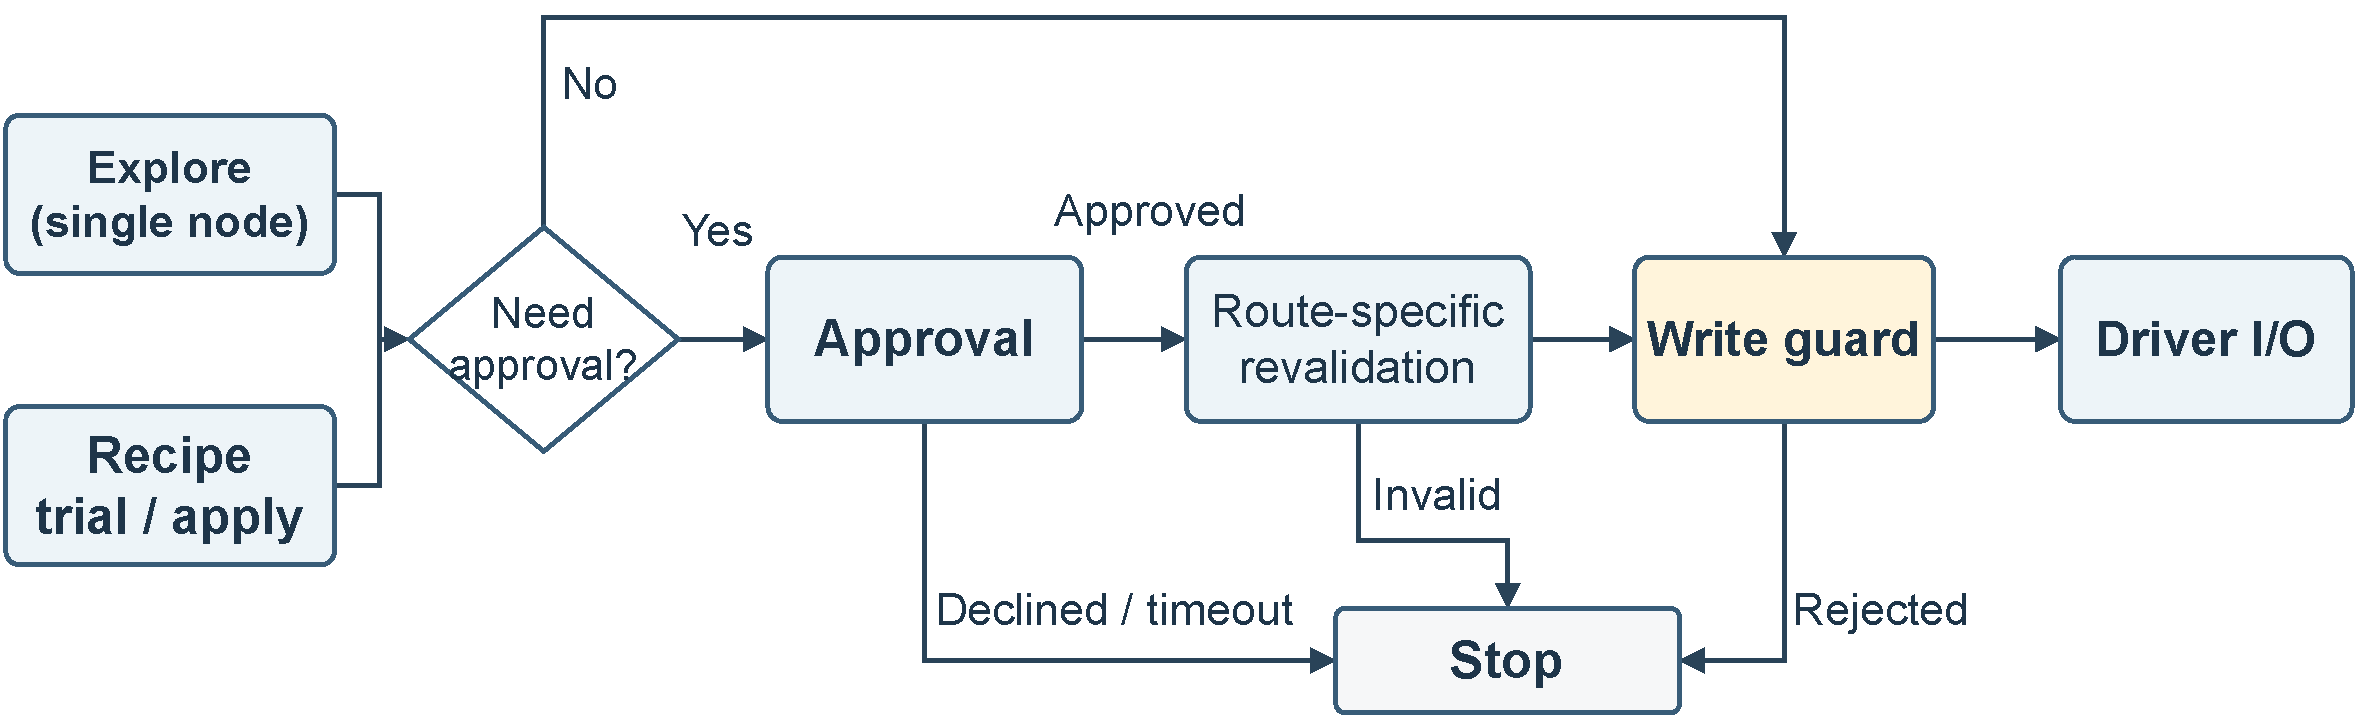
\includegraphics[width=\columnwidth]{resources/fig4-governed-flow.pdf}
\caption{Route map of the governed write paths, complementing the single-node sequence in Algorithm~1. Single-node \texttt{optimization\_explore} intents and recipe trial or apply operations take route-specific approval and revalidation before converging on the shared write guard of Eq.~(\ref{eq:admission}). A decline, timeout, failed revalidation, or guard rejection stops the affected operation or parameter before driver dispatch; command outcomes, setpoint readbacks, and later observations remain distinct records. Other applicable dispatch and authorization checks are omitted; bypassing approval does not bypass them.}
\label{fig:hitl}
\end{figure}
Fig.~\ref{fig:hitl} maps both write routes onto the shared write guard and the distinct records returned after dispatch; Algorithm~1 details the single-node check sequence. For a manual single-node \texttt{optimization\_explore} request, approval covers the node, proposed value, current effective interval, and rationale. The same boundary receives an agent's typed intent after acquisition and analysis. As in Algorithm~1, a decline or timeout stops the request. Approval triggers revalidation of the original direct node binding or, for a recipe operation, the recipe binding and parameter membership. Single-node approval does not use the recipe-operation context snapshot described next. In either path, revalidation does not make the checks and external device write atomic.

Recipe operations use a separate approval path. For \texttt{recipe\_trial} and \texttt{recipe\_apply}, approval is bound to the recipe operation and
active line--product--recipe--run context. After approval, the handler checks
authority and context again and verifies the recipe definition and
candidate scope before dispatch. A changed context, revoked binding, or
changed recipe definition prevents that proposal from proceeding. Recipe
trial approvals default to a 30-minute window; single-node approval waits
expire after 180\,s. Outside benchmark mode, agent and manual
writes are subject to a minimum 60-s interval following a setpoint change;
recipe trials also use a per-line cadence of 300\,s by default.

A \texttt{recipe\_trial} submits a bounded batch from the agent's control intent through the configured
driver and returns a result for each parameter to the calling route. Parameters are attempted
individually, so a batch can be partially applied; results and device state must be reconciled before any retry. A trial does not save or apply a recipe
version, and before updating, applying, or rolling back the recipe, the caller can retrieve later DAQ observations separately.

As sketched in Fig.~\ref{fig:hitl}, receipts record the command outcome returned to the agent or caller; observations record what followed in
the process. Command results are graded as readback-verified,
transport-acknowledged, or unverified. When a successful recipe write is not
already readback-verified, the service may, by default, attempt up to three additional
reads at 2\,s intervals where supported; recipe batches retain verification
outcomes for each parameter. A readback-verified result means that the
returned value matched the request within the applicable tolerance. A transport
acknowledgment alone does not establish that the device applied the value, and
an unverified result does not establish a matching readback. DAQ stores later
timestamped process observations for the agent's next analysis turn, while
recipe history, approvals, and task records remain with their owning services.
Identifiers and timestamps can link these records when available, but a later
observation alone does not prove that the command caused the measured change.



\section{Experimental Evaluation}
\label{sec:eval}
We evaluated whether the runtime routed a request to the configured simulator setpoint, blocked inadmissible values, and made the resulting process measurements available to the caller. The endpoint probes exercise node mappings and their guards. The scripted runs use the agent-tool interface to alternate acquisition and recipe trials. Separate fixtures test approval and production-mode checks, and three language-model episodes show what the agent path completed.

The integrated runs used already-running services. Benchmark mode bypassed step, interval, and hold-window checks for agent and manual writes. We exercised those checks separately in production mode. All equipment responses reported here came from simulators or mock drivers.

\subsection{Configured Mapping and Integration Checks}
\label{sec:eval-mapping}
Two integrated executions at seed~42 each passed 77 assertions across 17 phases without an agent harness. A separate cast-film preset check on the same runtime configured five endpoint types and rejected all nine negative probes.

The retained November 6 matrix used the administrative node-write interface at 55 endpoints in four simulated scenes. It covered Modbus over Transmission Control Protocol (TCP), Modbus remote terminal unit (RTU), OPC UA, MQTT, and Hypertext Transfer Protocol (HTTP). Per endpoint, the runner submitted three interior values and the upper configured recipe-window bound, then tested values outside the recipe window and the hard engineering range. The common $-50$ candidate fell inside the biaxial dew-point range and was filtered before submission. The runner counted acceptance when the service returned HTTP~200 without an explicit unsuccessful outcome. On readable nodes, it issued a separate read after each admissible request and compared the simulator value with the request using the configured tolerance.

Table~\ref{tab:scene-probe-results} reports 220 accepted requests, 219 hard-range rejections, and 110 recipe-window rejections. Each of the 54 readable endpoints returned four distinct values in request order, for 216 matching readbacks. For example, the injection holding pressure read back 65~bar over OPC UA, the wastewater blower 35~Hz and the annealing zone~2 setpoint 725~$^\circ$C over Modbus TCP, and the biaxial drying setpoint 160~$^\circ$C over OPC UA. The corresponding injection probe at 102.8~bar was within the hard range and failed the recipe-window check. The one configured HTTP endpoint accepted all four corona-power requests, including 4.3~kW, and offered no actuator readback. Probe values and guards used the same scene configuration.

\begin{table*}[!t]
\centering
\caption{Outcomes of the retained scene--protocol probes. Denominators give the number of submitted probes or available follow-up reads in each class.}
\label{tab:scene-probe-results}
\footnotesize
\setlength{\tabcolsep}{3pt}
\begin{tabularx}{\textwidth}{@{}>{\raggedright\arraybackslash}p{1.55cm}r X r r r r@{}}
\toprule
Scene & Endpoints & Protocols represented & Accepted & Hard-range rejects & Recipe-window rejects & Matching reads \\
\midrule
Injection & 11 & TCP 5, RTU 2, OPC UA 3, MQTT 1 & 44/44 & 44/44 & 22/22 & 44/44 \\
Wastewater & 7 & TCP 1, RTU 3, OPC UA 2, MQTT 1 & 28/28 & 28/28 & 14/14 & 28/28 \\
Annealing & 7 & TCP 3, RTU 2, OPC UA 1, MQTT 1 & 28/28 & 28/28 & 14/14 & 28/28 \\
Biaxial line & 30 & TCP 20, RTU 1, OPC UA 8, HTTP 1 & 120/120 & 119/119 & 60/60 & 116/116 \\
\bottomrule
\end{tabularx}
\end{table*}

\subsection{Exploratory Fixed-Horizon Simulator Contrast}
\label{sec:eval-optimization}
We compared a deterministic setpoint policy with no-write in injection molding, wastewater treatment, and annealing. The script read the scene's configured DAQ variables, selected a candidate using scene-specific rules, and sent one recipe parameter per \texttt{recipe\_trial} call. The lines used automatic approval policy, with the applicable recipe checks and limits in force. The script logged trial requests and available recipe-run identifiers, allowed the process to settle, and used subsequent measurements to decide the next step.

The target bands were $32.5\pm0.35$~g for part mass, $3.4\pm0.6$~mg/L for dissolved oxygen, and $95\pm6$~HV for Vickers hardness. Runs used a nominal horizon of 180~s for injection and 240~s for the other scenes, with nominal 1-s sampling. Each arm had a separate reset and had to start within the prescribed process-value window. Arm order was randomized within each scene--seed block. We computed integrated absolute error (IAE) by trapezoidal integration of the absolute deviation from the target between the first and last retained samples. Internal gaps of up to 5~s were linearly interpolated. Longer gaps invalidated the pair.

Nine of the 11 blocks in the later post-pilot batch met the reset, start, and sampling criteria. Wastewater seed~45 and annealing seed~46 were excluded because their no-write traces had gaps of 9 and 6~s, respectively. The scripted policy had lower IAE in all nine valid pairs (Table~\ref{tab:selected-iae}). Each scripted run recorded a sample in its target band, and all nine no-write runs stayed outside their bands. Restricting each pair to its common observed time interval preserved the direction of all nine contrasts.

\begin{table}[!t]
\centering
\caption{Selected fixed-horizon simulator contrasts. Positive $\Delta$IAE means lower retained-window accumulated absolute error under the scripted policy.}
\label{tab:selected-iae}
\footnotesize
\setlength{\tabcolsep}{3pt}
\begin{tabular}{@{}lcc@{}}
\toprule
Scene (unit of $\Delta$IAE) & Valid & Median (range) \\
\midrule
Injection (g\,s) & 3/3 & 165.165 (162.535--195.169) \\
Wastewater ((mg/L)\,s) & 3/4 & 615.605 (611.670--630.980) \\
Annealing (HV\,s) & 3/4 & 8000.450 (7930.200--8084.150) \\
\bottomrule
\end{tabular}
\end{table}

The mission records show how the script used the route in each scene. At injection seed~44, it requested 58.31~bar from 45~bar and then 10.67~s from 6~s of holding time. The final post-settling mean was 32.163~g. At wastewater seed~43 the blower request went from 26 to 30.02~Hz, followed by further blower and dosing trials, and final dissolved oxygen was 3.620~mg/L. At annealing seed~43 the first zone~3 request went from 730 to 850~$^\circ$C. The script then adjusted zone~2 and line speed and recorded a final hardness of 98.92~HV. These sequences pair the script's recorded requests with its subsequent measurements. The archive lacks an aligned per-request driver journal for these runs.

Fig.~\ref{fig:optimization-trajectory}(a) shows that injection samples entered the target band within 15~s in all three scripted runs. Fig.~\ref{fig:optimization-trajectory}(b) lists their recorded starting and requested setpoints, including a second pressure request after the hold-time request for seed~46. Panels~(c)--(e) show the IAE for all nine valid pairs. An earlier valid injection seed-44 pair had an IAE difference of 193.320~g\,s, compared with 165.165~g\,s in the later repeat. The archive does not identify a pre-specified rule for choosing between batches. Supplementary File~S7 describes the exclusions and retained records.

\begin{figure*}[!t]
\centering
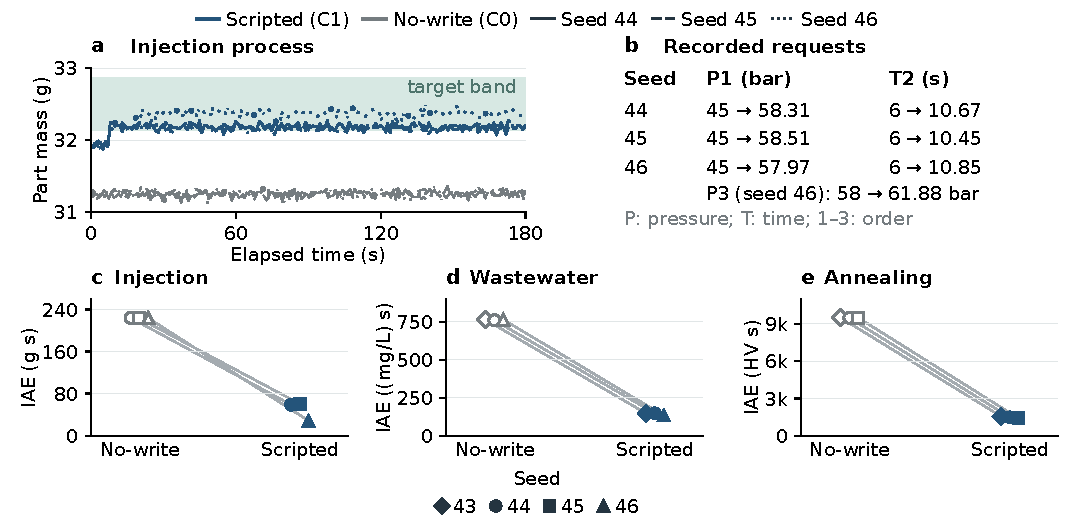
\includegraphics[width=\textwidth]{resources/fig5.pdf}
\caption{Scripted policy (C1) and no-write (C0) in the reported simulator batch. (a) Injection part-mass samples with the 32.15--32.85~g band shaded. Gaps over 1.5~s appear as breaks, and dots mark isolated samples. (b) Starting and requested setpoints from the script log. P and T denote hold pressure and hold time, and subscripts give request order. (c)--(e) Retained-window IAE for the nine valid pairs on scene-specific scales. Each line connects one seed pair. Small horizontal offsets separate overlapping markers.}
\label{fig:optimization-trajectory}
\end{figure*}

\subsection{Write-Guard and Route Behavior}
\label{sec:eval-ablation}
We tested the process-window check with a mock driver in one simulated scene. Four configurations combined enabled or disabled process-window and readback checks while retaining the hard range. Each configuration used three repetitions of four hard-range violations, two window violations, three legal values, and three boundary values. The violation values varied by configuration. Timed writes were counted separately.

Every configuration rejected all 12 hard-range violations and accepted all nine legal values. Enabling the window check rejected all six window violations per configuration. Disabling it let all six pass. Each configuration met all nine of its boundary expectations (Fig.~\ref{fig:guard-approval-results}(a)). This fixture measured service responses without injecting a readback mismatch.

A separate readback-fault probe returned 251 for a command of 230 with a tolerance of 0.7. The service returned HTTP~200 with an unsuccessful outcome graded \texttt{unverified}. A separate read of the simulator returned 251 as well. The baseline and recovery calls both returned \texttt{readback-verified}. In production mode, single tests of the interval, step, hard range, recipe window, and hold window all rejected the inadmissible request and the legal baseline passed. Authorization checks blocked unbound and cross-node requests and accepted the bound write.

The approval fixture submitted four \texttt{optimization\_explore} requests for injection barrel zone~1 temperature. A scripted approval permitted the setpoint to change from 202 to 204.8~$^\circ$C. A decline left it at 216~$^\circ$C. With approval disabled, the two requests changed 202 to 204.8~$^\circ$C and 216 to 218.8~$^\circ$C (Fig.~\ref{fig:guard-approval-results}(b)). The recorded pairing labels did not align with the starting temperatures, so we report the calls individually.

\begin{figure*}[!t]
\centering
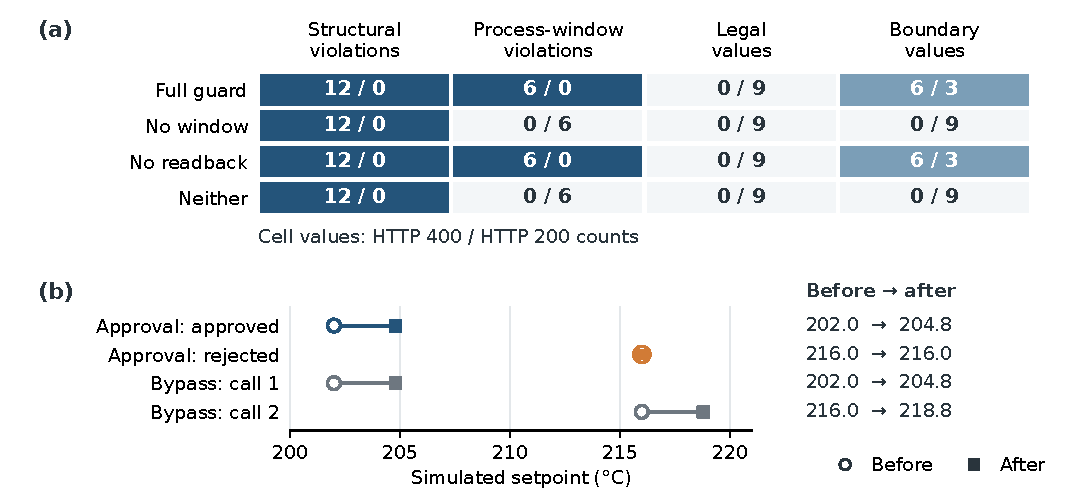
\includegraphics[width=\textwidth]{resources/fig6.pdf}
\caption{Guard and approval results. (a) HTTP~400/200 response counts for four guard configurations and four request classes. Shading gives the rejection proportion. Boundary expectations follow each configuration. (b) Simulated barrel-temperature setpoints before (circles) and after (squares) four separate requests. A scripted proxy supplied approval decisions where required.}
\label{fig:guard-approval-results}
\end{figure*}

\subsection{Injection-Twin Demonstration}
\label{sec:eval-twin-pilot}
An acceptance script submitted a three-step holding-pressure plan to an injection simulator. The execution service refused the pending plan until a scripted approval released it. After the three planned steps completed, a separate governed command changed holding pressure from 60 to 63.7~bar and the readback matched at 63.7~bar. After a 60-s wait, the last three 15-s DAQ buckets averaged 32.224~g, within the twin's 32.00--32.30~g band. Supplementary File~S7 records the baseline discrepancy and missing raw series for this single demonstration.

\subsection{LLM-Driven Simulator Episodes}
\label{sec:eval-agent}
Three injection episodes used the \texttt{deepseek-flash} model endpoint. Each worker trace contains a two-parameter recipe trial with automated approval and a response reporting both settings as verified. Separate episode-end platform snapshots show the same pressure and time values: 53~bar and 8~s, 54.8~bar and 8.2~s, and 56.6~bar and 8.4~s. The server-side driver journal and served model snapshot identifier were unavailable. All three tasks were canceled below the 32.15--32.85~g target band, at 31.70, 31.87, and 31.99~g, respectively. One episode recorded a process-quality guard flag.


\section{Discussion}
\label{sec:discussion}
The intended agent-mediated sequence---acquisition, objective-conditioned analysis, typed intent, governed dispatch, and reassessment of returned evidence---becomes explicit in the runtime (Section~\ref{sec:closed-loop-operation}). The selected fixed-horizon batch had lower retained-window error under the deterministic policy than under no-write in all nine valid blocks; Section~\ref{sec:eval} details the comparison's exploratory limits.

The evaluated runtime supports a concrete envelope of functions. Scene configuration binds production context to direction-specific acquisition and control mappings and registered protocol drivers; both entry paths meet at one dispatcher. Typed control intents pass execution-mode, authorization, write-limit, conditional-approval, and route-specific revalidation checks; outside benchmark mode, step, interval, and hold-window guards apply as well. Governed exploration and recipe-trial routes return command outcomes, readbacks, and later DAQ observations as separate, verification-graded records. Section~\ref{sec:eval} exercised this envelope across four simulated scenes and five protocols. The loop itself, however, has not been executed end-to-end by an autonomous agent: iteration still requires a subsequent agent decision, and all three language-model-driven episodes were canceled below target. The runtime therefore delivers a governed execution boundary. The closed-loop control mechanism---iterative acquisition, adjustment, and reassessment---is not yet realized in operation.

Fig.~\ref{fig:optimization-trajectory} presents the recorded injection mass traces and setpoint requests alongside the selected IAE contrasts; iteration-level timing and per-request server records are unavailable, so causal effects are not established. The mapping and guard tests support only the exercised branches; their oracles share configuration with the tested limits, and simulator readback is not physical actuation evidence. The LLM-driven episodes returned acknowledged updates but ended below target, and without the server journal cannot establish a complete agent-to-device write chain.

A complete immutable service and configuration snapshot was not retained. Further process validation requires a larger pre-specified study with verified reset states, common sampling and horizons, a named controller baseline, and complete trajectories; agent evaluation requires a fixed acquisition-and-control task, retained model and runtime versions, and correlated observation-to-intent-to-device records; human-approval effects and physical safety need separate studies.

Two extensions follow, and both remain future work. The first is autonomous closed-loop optimization through agent-architecture orchestration: a lead agent decomposes an objective, dispatches governed exploration or recipe steps, and reassesses returned evidence until a stopping rule is met---with every write still passing the same dispatch, approval, and revalidation checks. The second is process-experience memory reuse: validated scene-specific experience---operating context, applied intents, and observed outcomes---would accumulate and condition later proposals. Neither extension alters the boundary invariants. Both would inform proposals and sequencing only, granting no write authority.

\section{Conclusion}
\label{sec:conclusion}
This work presents a configuration-driven runtime for agent-mediated online data acquisition and governed setpoint control. It binds production context and direction-specific acquisition and control signals, returns observations for objective-conditioned analysis, and carries a typed control intent through route-dependent checks before dispatch, keeping command outcomes, readbacks, and later observations distinct. Mapping and guard branches were exercised in simulated scenes and mock-driver fixtures; all nine valid fixed-horizon scene--seed pairs had lower retained-window IAE under the scripted policy than under no-write, subject to the unresolved batch-selection rule and absent controller baseline, and the three LLM-driven episodes were canceled below target without a complete server-side write record. The evidence establishes an application-level agent-to-operation integration boundary, not autonomous closed-loop control, general optimizer convergence, a complete agent-to-device trace, or physical-plant safety. Realizing autonomous closed-loop operation through agent-architecture orchestration, with reuse of accumulated process experience to condition later proposals, is future work that must remain inside this governed boundary.


\section*{Declarations}
The authors declare no competing interests. The study used simulated scenes, mock drivers, and a programmable logic controller simulator. It involved no human participants, personal data, or physical-plant data. Author contributions and funding are withheld during anonymous review. The narrative supplement and supporting-evidence archive describe the experimental records.

\section*{Acknowledgment}
OpenAI Codex assisted with source organization, English editing throughout the manuscript, and redrafting the abstract and experimental narrative from the recorded evidence.

\bibliographystyle{IEEEtran}
% \IEEEtriggeratref{10} removed 2026-11-13: with the longer data-availability
% statement the forced break spilled the remaining references onto an 11th
% page; natural flow ends on page 10.
\bibliography{resources/refs}

\end{document}

